% ============================================================================
% Section 4 -- design. SECOND REWRITE 2026-09-07.
%
% The first rewrite added an architecture figure but was still hard to read:
% one static component diagram, dense prose, nothing concrete. A reader could
% not picture the compaction, could not see why k slots hide the transfer, and
% could not follow a request through the system.
%
% This version leads with four figures that carry the explanation:
%   fig:arch      the data path (components + who talks to whom)
%   fig:compact   the compaction, WORKED WITH REAL BLOCK IDS
%   fig:pipeline  the per-layer timeline -- why k>1 hides the transfer
%   fig:lifecycle a request's states and what triggers each transition
% Prose is trimmed to what the figures do not already say.
% ============================================================================

% PROVENANCE: the numbers in this section are design constants ($k{=}4$,
% $L{=}64$) or engine timings taken during development, as in
% \S\ref{sec:impl}. Measured results all live in \S\ref{sec:eval}, which
% carries the % src: comments.
\section{Design: five pillars, and what each one buys}
\label{sec:design}

\subsection{Overview}
\label{sec:design:overview}

Each request has a \emph{tier}: a \textbf{device-tier} request behaves exactly as
in stock vLLM, while a \textbf{host-tier} request holds \textbf{no blocks in the
device pool at all}. What follows is how that is possible --- why the host tier
needs its own address space, what a step does, and how the cohort is sized.
Appendix~\ref{app:figures} collects the notation, a component diagram and the
request-lifecycle state machine.

The design rests on five mechanisms. None is individually novel; what matters is
that each is load-bearing, and we can say by how much, because every one was
measured by removing it. Table~\ref{tab:pillars} is that accounting, and it is
also the honest answer to ``why does this work'' --- the first two pillars create
the opportunity, the next two make the overhead small enough to collect it, and
the last decides where to stand.

\begin{table}[t]
\centering
\small
\begin{tabular}{llcr}
\toprule
Pillar & Removing it costs & measured at & \S \\
\midrule
One forward, two KV sources & the whole gain & --- & \ref{sec:design:exec} \\
Transfer hidden under compute & $c$: $0.92 \to 7.20$\,ms & $L{=}64$, ctx 512 & \ref{sec:design:step} \\
$O(r)$ extent allocation & $c$: $1.26 \to 5.17$\,ms & $L{=}80$, ctx 8192 & \ref{sec:design:spaces} \\
Deferred, batched mirror write & $F$: $3.4 \to 13.4$\,ms & $L{=}64$, ctx 128 & \ref{sec:design:mirror} \\
Overhead-aware admission & $18\%$ of the gain & $L{=}80$, ctx 8192 & \ref{sec:design:admission} \\
\bottomrule
\end{tabular}
\caption{The five pillars and the measured cost of removing each. Every row is an
ablation, not an estimate. \textbf{The third column is load-bearing: these numbers
are not comparable to one another and are not meant to be.} Each ablation was run
against the configuration current when that mechanism was built, so the $c$ rows
differ in both depth and context, and neither is the $c$ of Eq.~\ref{eq:coeffs},
which is the \emph{final} coefficient measured below the knee at $L{=}64$
($0.49$\,ms). What each row licenses is the claim that its mechanism is necessary;
the deficits do not sum, and only Eq.~\ref{eq:coeffs} and
Fig.~\ref{fig:coeffs} should be read as the coefficients of the shipped system.}
% src: paper/data/overhead/15_clean_cf/CF_c128_a.json,
% paper/data/overhead/08_opt/T1_c2048_bs16.json,
% paper/data/overhead/19_t8/T8_on_a.json, paper/model/operating_point.py
\label{tab:pillars}
\end{table}

\subsection{Where the two tiers run}
\label{sec:design:exec}

%% Extracted from D-figures.tex 2026-10-08 so it can sit in the
%% BODY, beside the text that discusses it, rather than in an
%% appendix. Exactly one definition: D-figures.tex no longer has
%% a copy.
\begin{figure}[t]
\centering
\resizebox{\columnwidth}{!}{%
\begin{tikzpicture}[
  x=1cm, y=1cm, font=\scriptsize,
  op/.style={draw, rounded corners=2pt, align=center, minimum height=7mm,
             minimum width=2.2cm, inner sep=1.2mm, fill=black!5},
  at1/.style={op, fill=black!8, minimum width=2.8cm},
  at2/.style={op, fill=blue!12, draw=blue!45, minimum width=2.8cm},
  lbl/.style={font=\scriptsize\itshape, text=black!60, align=center},
  arr/.style={-{Latex[length=1.5mm]}},
]
\node[op] (qkv) at (0,0) {QKV projection\\{\scriptsize all $B$ rows}};
\node[at1] (a1)  at (3.5,0.8) {flash \#1: all rows\\{\scriptsize vs paged pool}};
\node[at2] (a2)  at (3.5,-0.8) {flash \#2: host rows\\{\scriptsize vs slot $\ell\bmod k$}};
\node[op] (o)   at (7.0,0) {O-proj, MLP\\{\scriptsize all $B$ rows}};
\draw[arr] (qkv) -- (a1);
\draw[arr] (qkv) -- (a2);
\draw[arr] (a1) -- (o);
\draw[arr] (a2) -- (o);
\node[lbl] at (0,-1.1) {weights read once};
\node[lbl] at (7.0,-1.1) {weights read once};
\node[lbl, text=blue!70] at (3.5,-1.85)
     {\#1 masks host rows to a single key;\\
      \#2 gathers them, attends the slot, scatters back};
\end{tikzpicture}}
\caption{\textbf{One layer, one forward pass.} Every operation except attention
runs once over the whole batch, so a host-tier request adds a row to GEMMs that
are memory-bound on the weights regardless. Attention is two \emph{sequential}
kernel launches over disjoint row subsets of the same tensors --- not a spatial
partition of the device.}
\label{fig:exec}
\end{figure}


\textbf{There is no partition of the GPU.} The two tiers are not separate streams,
kernels or forward passes but \emph{rows of the same batch}; the only operation that
distinguishes them is attention, and only in \emph{where it reads keys and values
from} (Fig.~\ref{fig:exec} draws one layer). Three consequences follow. Everything
but attention is shared, so a host-tier request adds one row to GEMMs that are
memory-bound on the weights regardless --- on an 8B model until batch 142
(Appendix~\ref{app:params}). The two attention calls are sequential on the same
hardware, so they do not compete for SMs, and the second's cost scales with the
host-tier rows rather than the batch. And the first does no wasted work for those
rows: masking their \texttt{seqused\_k} to 1 makes them attend a single key and be
overwritten by the second, worth 22\% of wall time. So a host-tier request occupies a
row in a step that was happening anyway, paying its KV read out of interconnect
bandwidth idle while the step reads weights --- the sense in which it rides along.

\textbf{What it buys: the entire numerator.} Every other pillar reduces a cost;
this one is why there is anything to collect. Because the weights are read once for
both cohorts, $r$ riders multiply throughput by $(1 + r/B_{\mathrm{cap}})$ at no
weight-read cost --- the term that pays for all the overhead below it. Serving the
cohorts as separate forward passes would read the weights twice and leave nothing.

\subsection{Why the host tier has its own addresses}
\label{sec:design:spaces}

The host mirror is \textbf{not} indexed by device block id, and the rest of the
design rests on that. Under vLLM's allocator, releasing a block nulls the owner's
block-table entry and returns the id to a free list from which it is promptly
reissued --- so a mirror keyed by device block id would both \emph{lose the read
mapping} and \emph{alias}, the reissued id now denoting another request's data. Each
\emph{(request, logical block)} therefore gets an id from a private host space, held
until the request finishes, and device ids may churn underneath. Growth needs no
device allocation either: a new logical block takes a fresh host block and its
tokens arrive through the per-layer write path.

The price is that the cohort's host ids are scattered while the rolling region is a
small dense array. A \emph{compaction} once per step bridges them, sorting the
cohort's blocks onto $[0,R)$ so every layer reuses one block table while the slot
contents rotate beneath it.

\textbf{What it buys: $c$ stops scaling with blocks.} The compaction must be
$O(r)$, not $O(\text{blocks})$. Building the block table one entry per rider-block
per step --- the obvious implementation --- made $c$ grow with context and put it
at $5.17$\,ms per rider, above the $3.37$\,ms a resident is worth, so \emph{no
interconnect at any bandwidth} could have paid. Allocating whole extents instead
leaves $0.0031$\,ms per rider with no context term at all, and is what moves the
design from arithmetically impossible to profitable.

\subsection{A decode step, end to end}
\label{sec:design:step}

%% Extracted from D-figures.tex 2026-10-08 so it can sit in the
%% BODY, beside the text that discusses it, rather than in an
%% appendix. Exactly one definition: D-figures.tex no longer has
%% a copy.
\begin{figure}[t]
\centering
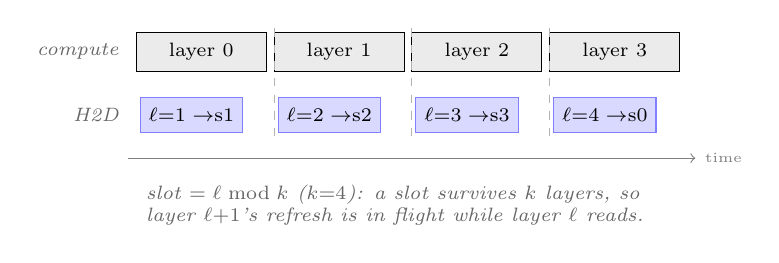
\begin{tikzpicture}[
  x=1cm, y=1cm, font=\scriptsize,
  cmp/.style={draw, fill=black!8, minimum height=5mm, inner sep=1pt},
  xfer/.style={draw, fill=blue!15, draw=blue!50, minimum height=4.5mm, inner sep=1pt},
  lbl/.style={font=\scriptsize\itshape, text=black!60},
]
\node[lbl, anchor=east] at (-0.1,0.2) {compute};
\foreach \i/\x in {0/0,1/1.75,2/3.5,3/5.25}
  \node[cmp, minimum width=1.65cm] at (\x+0.825,0.2) {layer $\i$};

\node[lbl, anchor=east] at (-0.1,-0.6) {H2D};
\foreach \i/\x/\s in {1/0/1,2/1.75/2,3/3.5/3,4/5.25/0}
  \node[xfer, minimum width=1.3cm] at (\x+0.70,-0.6) {$\ell{=}\i\rightarrow$s\s};

\foreach \x in {1.75,3.5,5.25} \draw[dashed, black!30] (\x,0.5) -- (\x,-0.95);
\draw[->, black!50] (-0.1,-1.15) -- (7.1,-1.15) node[right, font=\tiny] {time};

\node[lbl, anchor=west, align=left] at (0,-1.75)
  {slot $= \ell \bmod k$ ($k{=}4$): a slot survives $k$ layers, so\\
   layer $\ell{+}1$'s refresh is in flight while layer $\ell$ reads.};
\end{tikzpicture}
\caption{\textbf{Per-layer pipeline.} The refresh for layer $\ell{+}1$ is issued
while layer $\ell$ computes. $k$ slots give a transfer $k{-}1$ layers of slack
before its destination is reused, which is what allows it to be hidden;
$k{=}1$ would serialise transfer against compute. \S\ref{sec:eval:cost}
measures the fraction actually hidden.}
\label{fig:pipeline}
\end{figure}


Two granularities matter, and separating them keeps the per-layer work small:
\textbf{addresses} are fixed for the whole step, while slot \textbf{contents} change
every layer. Once per step, compact. Per layer, issue the runs into rolling slot
$\ell \bmod k$ --- with $k>1$ issued ahead, so layer $\ell{+}1$'s transfer overlaps
layer $\ell$'s compute, which is the hiding window the design turns on. Per layer,
attend: device-tier rows read the paged pool with the ordinary block table,
host-tier rows read slot $\ell \bmod k$ with the compacted one, in one pass over
shared weights. Per layer, write: the new $K,V$ for host-tier rows go to the
authoritative host mirror \emph{and} into the current slot, so this step's own
attention sees them. Several transitions are driven by the \emph{worker} rather than
the scheduler, which is not incidental: the scheduler cannot observe a host-side
write, so anything conditioned on KV having arrived must wait for an acknowledgement
(Appendix~\ref{app:figures}).

\textbf{What it buys: the bytes become free.} The $k>1$ lookahead is the pillar the
whole premise rests on, and it is not a marginal optimisation: with it $c = 0.92$\,ms
per rider, without it $7.20$\,ms, which fails the $3.37$\,ms budget by more than
twofold. Run deep enough below the knee and the transfer disappears from the step
entirely --- removing a rider's bytes while keeping every launch moves $c$ by
$0.010$\,ms. \textbf{That is the result that reframes the design}: what a faster
interconnect buys is not a cheaper rider but a higher knee
(\S\ref{sec:model:knee}), and $c$ is left holding only launch and bookkeeping work.

\subsection{The mirror write, deferred and batched}
\label{sec:design:mirror}

The host mirror is authoritative, so each step's new $K,V$ must reach it. Doing
that per layer, synchronously, is the single largest avoidable cost in the design:
a blocking pageable copy once per layer put $F$ at $13.4$\,ms, $85\%$ of it in that
one operation, and at $71\,\mu$s per copy it cost $446\times$ the transfer it
performed. Deferring the writes and flushing them as one batched scatter per step
--- two vectorised index-copies rather than $2L$ --- takes $F$ to $3.4$\,ms.

\textbf{What it buys: $F$, which is now the binding constraint.} With $c$ clearing
its budget fivefold, the fixed cost is the only term that decides the margin, so
$74\%$ of $F$ removed is the difference between the thin result this paper
originally reported and Table~\ref{tab:gain}. Two cautions belong with it. The
largest single saving came from finding that a \emph{disabled} feature was flushing
the batch on every layer, which had silently defeated the batching since the day it
landed --- the overhead was not where the design said it was. And of the $3.4$\,ms
that remains, $1.2$ is the extra attention call of \S\ref{sec:design:exec}, which
Appendix~\ref{app:ridercost} prices by ablation rather than projecting: fusing the
two calls is worth between $+2$ and $+8.5$ points, and we decline to spend days of
backend work against the lower end of that range until one cheap off-engine
measurement narrows it.

\subsection{Admission}
\label{sec:design:admission}

Each host-tier request costs $S\btok$ bytes of interconnect per step, and
admission bounds their sum by the step time times the achieved bandwidth, less a
margin. Three scheduler behaviours must then agree for such a request to hold no
device blocks, and all three are necessary. \emph{Admission without allocation}:
the request enters with an empty block list, its KV having been delivered into
the host pool by the prefill transport (\S\ref{sec:background:pd}), contingent on
the worker's acknowledgement. \emph{No prefill allocation}: its prompt is marked
already computed, so nothing is allocated even transiently --- the batch is
bounded by \emph{peak} device residency, so allocating during prefill and
reclaiming afterwards still pays the peak. \emph{Queue bypass}: vLLM's waiting
queue stops at the first request it cannot allocate for, so a block-starved
request ahead would otherwise block an admission that needs no resources.

\textbf{What it buys: $18\%$, from configuration alone.} Admission must respect
Eq.~\ref{eq:knee} and, because riders are integers, must round \emph{down}: a
budget that admits $1.89$ riders admits one. Choosing the operating point with that
in mind is worth more than every code change above combined --- $\times 1.25$
against $\times 1.07$ for the same model and hardware at a context $5\%$ shorter
(\S\ref{sec:model:knee}), where the whole remaining optimisation programme we can
identify is bounded at $+14\%$ and most of that is unreachable. It is also the one
pillar whose benefit needs no new mechanism, only a policy that knows the knee,
which is why we treat the overhead law rather than the transport as this paper's
contribution.

\subsection{Placement and migration are mechanisms, not contributions}
\label{sec:design:placement}

\S\ref{sec:model} fixes \emph{how many} bytes each tier carries without reference
to which requests supply them: in the fluid limit, freed device memory and spent
interconnect both scale with $S\btok$, so any assignment filling both budgets
realises the whole gain. Placement can matter only through what that limit omits
--- integer effects at long context, remaining lifetime, KV growth, migration
cost, recompute-preemption --- so we present it as a mechanism the manager needs
rather than as a result.

The intuitive signal is the wrong one. \textbf{Context length does not discriminate
to first order}: moving a request of context $S$ frees $S\btok$ bytes and costs
$S\btok$ bytes every step, so ranking by context is ranking arbitrarily. What
survives is \emph{remaining} generation, which sets how many steps a one-time seed
amortises over. Placement must also be revisable --- blocks free when a resident
finishes, and a cohort that outgrows the pool is worth demoting whenever that costs
less than the recompute-preemption it avoids --- so both moves carry hysteresis and a
cooldown. The gate cannot be the byte budget alone, since the host path also carries
a fixed per-step cost, so a demotion is a \textbf{probe}: make the move, settle,
compare on \emph{goodput} rather than latency, because a demotion always lengthens
the step while its benefit is requests served. Appendix~\ref{app:figures} gives the
estimator and the thresholds; \S\ref{sec:eval:ablation} explains why a two-rider
budget cannot test any of it.
\label{sec:design:migration}
